% \begin{lstlisting}
% 可用的模拟器:
% 1. 态矢量(强调 little endian)
% 2. 密度矩阵
% 3. 张量网络

% 使用方法:
% 1. apply_gate
% 2. apply_circuit
% 3. apply_hamiltonian(介绍mq中的Hamiltonian)
% 4. get_expectation
% 5. get_expectation_with_grad
% 6. sampling
% \end{lstlisting}
View demo code of this section: \democode{02}{2.6}

There are many methods to simulate a quantum system. For example, you can use a full state vector to simulate a pure quantum system and use a density matrix to simulate a mixed state quantum system. In \MindQuantum, both of these methods are supported.

\begin{lstlisting}
from mindquantum.core.gates import H
from mindquantum.simulator import Simulator

sim = Simulator('mqvector', 2)
sim.apply_gate(H.on(0))
print(sim)
\end{lstlisting}
The output is:

\begin{lstlisting}
mqvector simulator with 2 qubits (little endian), dtype: mindquantum.complex128.
Current quantum state:
√2/2¦00>
√2/2¦01>
\end{lstlisting}

In the above demo, we initialized a full state vector simulator named `mqvector', which is a full state quantum simulator. Up to version 0.9.0, all simulator that \MindQuantum supported is shown as below:
\begin{table}[ht]
    \begin{tabular}{ccccc}
        \toprule
        Name          & CPU & GPU & Complex64 & Complex128 \\
        \midrule
        mqvector      & Yes & No  & yes       & yes        \\
        mqvector\_gpu & No  & Yes & yes       & yes        \\
        mqmatrix      & Yes & No  & yes       & yes        \\
        \bottomrule
    \end{tabular}
    \caption{Supported quantum simulator.}
    \label{tab:simulator_supported}
\end{table}
After applying a hadamard gate, we gate a quantum state $\left(\ket{00}+\ket{01}\right)/\sqrt{2}$. What we need to emphasize is that in the whole framework, we use little endian notation, that is, for base $\ket{01}$, the first qubit is in state $\ket{1}$ end the second qubit is in state $\ket{0}$.

Every simulator in \MindQuantum maintains a quantum state, and we can use methods start with `apply' to change the quantum state and use methods start with `get' to extracting information from the quantum state.

\subsubsection{`apply' method}

`apply' method is going to applying a operator on the maintained quantum state and change the state. We a apply a single gate or a quantum circuit on the quantum state, and we can also apply a hamiltonian on the quantum state. We should notice that after applying a hamiltonian, the quantum state will not be a will defined quantum state.

\begin{lstlisting}
from mindquantum.core.circuit import Circuit
from mindquantum.core.operators import Hamiltonian, QubitOperator
from mindquantum.simulator import Simulator

circ = Circuit().h(0).x(1, 0)
ham = Hamiltonian(QubitOperator('X0 Y1'))
sim = Simulator('mqvector', 2)
sim.apply_hamiltonian(ham)
sim.apply_circuit(circ)
\end{lstlisting}
The output is:
\begin{lstlisting}
mqvector simulator with 2 qubits (little endian), dtype: mindquantum.complex128.
Current quantum state:
-√2/2j¦01⟩
√2/2j¦10⟩
\end{lstlisting}

\subsubsection{`get' method}

`get' method will not change the maintained quantum state but extract useful information.

1. \getqs

You can get the quantum matrix or a ket string expression (with arg \code{ket=True}) from a simulator with this method.
\begin{lstlisting}
from mindquantum.algorithm.library import qft
from mindquantum.simulator import Simulator

sim = Simulator('mqvector', 3)
sim.apply_circuit(qft(range(3)))
qs = sim.get_qs()
print(sim.get_qs(ket=True))
\end{lstlisting}

2. \getexpectation

Calculating the expectation of a given observable is a very common requirement. In \MindQuantum, we expand the definition of observable to below:

\begin{equation}
    E = \bra{\varphi}U_l^\dagger H U_r \ket{\psi}
\end{equation}

Following this definition, we are easily to get the physical observable if we set $\ket{\varphi}=\ket{\psi}$ and $U_l = U_r$ and we cal also to calculate the inner product of two quantum state if we set $H=I$

\begin{lstlisting}
from mindquantum.core.circuit import Circuit
from mindquantum.core.operators import Hamiltonian, QubitOperator

# Get expectation
psi = Simulator('mqvector', 2)
H = Hamiltonian(QubitOperator('Z0 Z1'))
U_r = Circuit().rx(2.5, 0)
psi.get_expectation(H, U_r)

# Get inner product
phi = Simulator('mqvector', 2)
H = Hamiltonian(QubitOperator(''))
U_l = Circuit().ry(1.5, 0)
psi.get_expectation(H, U_r, U_l, phi)
\end{lstlisting}

\subsubsection{sampling}

Quantum sampling is a fundamental aspect of quantum computing that plays a pivotal role in solving certain complex problems efficiently. It leverages the principles of quantum superposition and entanglement to explore multiple possibilities simultaneously, enabling quantum computers to outperform classical counterparts in specific scenarios.

In \MindQuantum, we can use a simulator to sample the measurement result of a quantum circuit.
\begin{lstlisting}
from mindquantum.utils import random_circuit
from mindquantum.simulator import Simulator

circ = random_circuit(3, 5, seed=42)
circ.barrier().measure_all()
sim = Simulator('mqvector', circ.n_qubits)
res = sim.sampling(circ, shots=1000, seed=42)
\end{lstlisting}

\begin{figure}[h]
    \begin{center}
        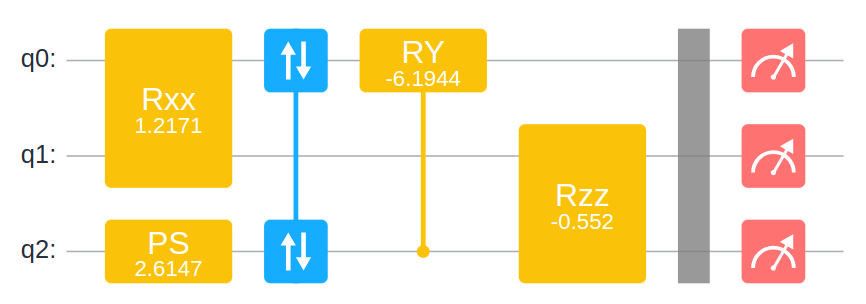
\includegraphics[width=0.9\linewidth]{images/2_6_sampling_circ.png}
    \end{center}
    \caption{Sampling circuit}
\end{figure}

\begin{figure}[h]
    \begin{center}
        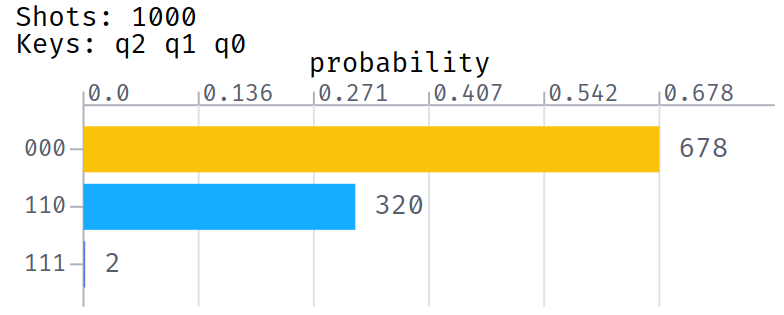
\includegraphics[width=0.9\linewidth]{images/2_6_sampling_res.png}
    \end{center}
    \caption{Sampling result}
\end{figure}
